\documentclass[aspectratio=169]{beamer}
\usepackage[T1]{fontenc}
\usepackage[utf8]{inputenc}
\usepackage{listings}
\usepackage{xcolor}
\usepackage{hyperref}
\usepackage{graphicx}
\usepackage{textcomp}
\usepackage{tikz}
\usepackage{tcolorbox}
\usepackage{menukeys}
\usepackage{pdfpages}

\tcbuselibrary{listings}

\usefonttheme[onlymath]{serif}

\usecolortheme[RGB={37,68,113}]{structure}
\usetheme{Dresden}

% generic colors
\definecolor{dirblue}{HTML}{9bc1ff}

% TheAlternative colors
\definecolor{ldorange}{HTML}{F18A20}
\definecolor{ldblue}{HTML}{254471}

%Apply TheAlt colors to theme
\setbeamercolor{section in head/foot}{fg=ldorange}
\setbeamercolor{author in head/foot}{fg=white}
\setbeamercolor{subsection in head/foot}{fg=white}
\setbeamercolor{caption name}{fg=vlg}
\setbeamercolor{caption}{fg=vlg}
\setbeamercolor{frametitle}{fg=ldblue}
\setbeamercolor{title}{fg=ldorange}
\setbeamercolor{institute}{fg=ldblue}
\setbeamertemplate{itemize item}[circle]
\setbeamercolor{itemize item}{fg=ldorange}

% make including pdfs work
\setbeamercolor{background canvas}{bg=}

\setbeamerfont{title}{series=\bfseries}

\setbeamertemplate{caption}{\raggedright\insertcaption\par}
\setbeamertemplate{navigation symbols}{}
\setbeamertemplate{bibliography item}[text]

% white-on-black lstlisting env with rounded corners
\newenvironment{bashenv}[1][\small]{%
    \tcblisting{listing only,colback=black,colframe=black,
        enlarge top by=0mm,left=-0mm,top=-2mm,bottom=-2mm,
        listing options={language=bash,
            escapechar=§,
            basicstyle=#1\color{white}\ttfamily,
            backgroundcolor=\color{black},
            breaklines=true,
            keepspaces=true,
            showstringspaces=false,
            columns=fullflexible}}}
{\endtcblisting}

% mark a spot for e.g. drawing an arrow to it
\newcommand\tikzmark[1]{\tikz[remember picture,overlay]\node[inner xsep=0pt](#1){};}

% \newcommand\Warning{%
%     \makebox[1.4em][c]{\raisebox{-0.45em}{%
%         \makebox[0pt][c]{\raisebox{0.25em}{\large!}}%
%         \makebox[0pt][c]{\color{red}\Huge$\bigtriangleup$}}}%
%         \hspace{0.7em}%
% }

% a red warning box
\definecolor{lred}{HTML}{ffd6dd}
\newtcolorbox{WarningBox}{%
    colframe=red,
    colback=lred}



\title{The Console Toolkit}
\author{Lukas Tobler}
\institute{TheAlternative, SSC | ETHZ and UZH}
\date{HS 2018}

\begin{document}
	\begin{frame}
		\titlepage%
	\end{frame}

    \section{Introduction}

    \begin{frame}[t,fragile]{Why the console? It's already current year!}
        \begin{itemize}
            \item People asked for it
            \item Still an excellent interface for complex tasks
            \item Many advanced tools only available on the command line
            \item Can be much faster than GUI tools
            \item Allows easy remote access to other computers
            \item Skills portable to every Unix-like system
        \end{itemize}
    \end{frame}

    \begin{frame}[t,fragile]{Course outline}
        \begin{columns}[T]
            \column{0.5\textwidth}
            \textbf{Part 1}
            \begin{itemize}
                \item Navigating the file system
                \item Modifiying files
                \item Working with text files
                \item Getting used to the console
            \end{itemize}
            \column{0.5\textwidth}
            \textbf{Part 2}
            \begin{itemize}
                \item{Users \& rights}
                \item{Managing software}
                \item{SSH}
                \item{Git}
                \item{Backups}
                \item{Scripting}
            \end{itemize}
        \end{columns}
    \end{frame}

    \begin{frame}[t,fragile]{What is the console}
        \begin{columns}[T]
            \column{0.4\textwidth}
            \begin{itemize}
                \item Keyboard-only interface to your computer
                \item Related terms: \emph{console}, \emph{terminal},
                    \emph{shell}, \emph{bash}, \emph{command prompt},
                    \emph{command line interface}
            \end{itemize}
            \column{0.6\textwidth}
            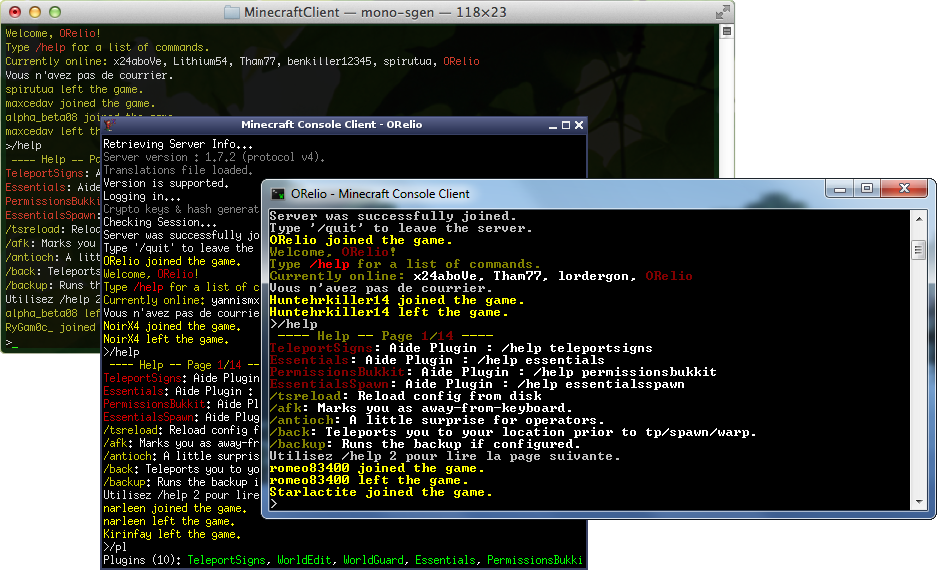
\includegraphics[width=\columnwidth]{img/consoles.png}
        \end{columns}
    \end{frame}

    \section{Navigation}

    \begin{frame}[t,fragile]{The 70s were interesting times, or so I'm told}
        \textbf{Unix dogma: \emph{Everything is a file!}} \\
        \begin{itemize}
            \item Data files
            \item Directories (or ``folders'')
            \item Storage devices
            \item Keyboards
            \item Printers
            \item Cameras
            \item \emph{But not network sockets \ldots}
        \end{itemize}
    \end{frame}

    \begin{frame}[t,fragile]{File system}
        \begin{columns}[T]
            \column{0.5\textwidth}
            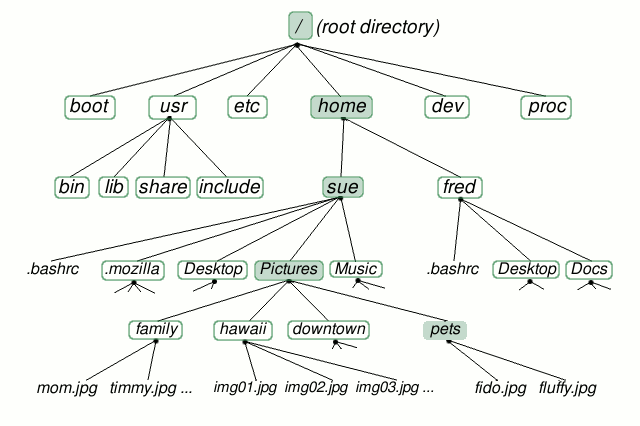
\includegraphics[width=\columnwidth]{img/dirtree.png}
            \column{0.5\textwidth}
            \begin{itemize}
                \item File system organized as tree
                \item Everything under \texttt{/}, the root directory
                \item In the console, you will be at some point in the tree,
                    the \emph{working directory}
            \end{itemize}
        \end{columns}
    \end{frame}

    \begin{frame}[t,fragile]{Working directory}
        \begin{columns}[T]
            \column{0.5\textwidth}
            \begin{itemize}
                \item Where am I? \textrightarrow \: \texttt{pwd}
                \item \underline{P}resent \underline{w}orking \underline{d}irectory
                \item Also sometimes directly shown in the prompt
            \end{itemize}
            \column{0.5\textwidth}
            \begin{bashenv}[\small]
[luke@host ~]$ pwd
/home/luke
[luke@host ~]$
            \end{bashenv}
        \end{columns}
    \end{frame}

    \begin{frame}[t,fragile]{Listing files}
        \begin{columns}[T]
            \column{0.5\textwidth}
            \begin{itemize}
                \item What is in here? \textrightarrow \: \texttt{ls}
                \item \emph{list}
            \end{itemize}
            \column{0.5\textwidth}
            \begin{bashenv}[\small]
[luke@host ~]$ ls
§\textcolor{dirblue}{Desktop}§
§\textcolor{dirblue}{Documents}§
§\textcolor{dirblue}{Downloads}§
§\textcolor{dirblue}{Music}§
§\textcolor{dirblue}{Pictures}§
§\textcolor{dirblue}{Videos}§
cat1.jpg
cat2.jpg
[luke@host ~]$
            \end{bashenv}
        \end{columns}
    \end{frame}

    \begin{frame}[t,fragile]{Commands \& arguments}
        \vspace{0.5cm}
        \texttt{\tikzmark{a}{l}s \tikzmark{b}{-}a
            \tikzmark{c}{-}-human-readable \tikzmark{d}{/}home/luke/pictures}\\
        \begin{tikzpicture}[remember picture,overlay]
            \node[align=left,xshift=0.4cm,yshift=-1.0cm,rounded corners,
            fill=red!20,draw=red!70!black] (b1)
            {\footnotesize{command}};
            \draw[red!70!black,->] (b1) edge ([yshift=-0.05cm,xshift=7.0pt]a.south);

            \node[align=left,xshift=3.0cm,yshift=-2.3cm,rounded corners,
            fill=green!20,draw=green!70!black] (b2)
            {\footnotesize{single letter option}};
            \draw[green!70!black,->] (b2) edge ([yshift=-0.05cm,xshift=9.5pt]b.south);

            \node[align=left,xshift=3.7cm,yshift=-0.7cm,rounded corners,
            fill=green!20,draw=green!70!black] (b3)
            {\footnotesize{long option}};
            \draw[green!70!black,->] (b3) edge ([yshift=-0.05cm,xshift=1.5cm]c.south);

            \node[align=left,xshift=6.7cm,yshift=-0.7cm,rounded corners,
            fill=orange!40,draw=orange!70!black] (b4)
            {\footnotesize{arguments}};
            \draw[orange!70!black,->] (b4) edge ([yshift=-0.05cm,xshift=1.7cm]d.south);
        \end{tikzpicture}
    \end{frame}

    \begin{frame}[t,fragile]{Advanced listing}
        \begin{columns}[T]
            \column{0.5\textwidth}
            \begin{itemize}
                \item \texttt{ls} has advanced options
                \item \texttt{-a}: show hidden files
                \item \texttt{-h}: print numbers in human readable format
                \item \texttt{-l}: show the long output format.
                \item \texttt{ls -lah} and \texttt{ls -l -a -h} are
                    equivalent
            \end{itemize}
            \column{0.5\textwidth}
            \begin{bashenv}[\tiny]
[luke@arch-x270 ~]$ ls -lah
total 52K
drwx------ 8 luke luke 4.0K Sep  3 23:27 .
drwxr-xr-x 4 root root 4.0K Sep  3 23:26 ..
-rw-r--r-- 1 luke luke   21 Jun  4 10:54 .bash_logout
-rw-r--r-- 1 luke luke   57 Jun  4 10:54 .bash_profile
-rw-r--r-- 1 luke luke  141 Jun  4 10:54 .bashrc
-rw-r--r-- 1 luke luke    0 Sep  3 23:27 cat1.jpg
-rw-r--r-- 1 luke luke    0 Sep  3 23:27 cat2.jpg
drwxr-xr-x 2 luke luke 4.0K Sep  3 23:27 §\textcolor{dirblue}{Desktop}§
drwxr-xr-x 2 luke luke 4.0K Sep  3 23:27 §\textcolor{dirblue}{Documents}§
drwxr-xr-x 2 luke luke 4.0K Sep  3 23:27 §\textcolor{dirblue}{Downloads}§
-rw-r--r-- 1 luke luke   24 Sep  3 23:28 .hidden_file
drwxr-xr-x 2 luke luke 4.0K Sep  3 23:27 §\textcolor{dirblue}{Music}§
drwxr-xr-x 2 luke luke 4.0K Sep  3 23:27 §\textcolor{dirblue}{Pictures}§
-rw-r--r-- 1 luke luke 3.7K Oct 23  2017 .screenrc
drwxr-xr-x 2 luke luke 4.0K Sep  3 23:27 §\textcolor{dirblue}{Videos}§
[luke@arch-x270 ~]$
            \end{bashenv}
        \end{columns}
    \end{frame}

    \begin{frame}[t,fragile]{Getting help}
        \begin{itemize}
            \item Where can I find out what options are available?
            \item Manual pages!
            \item \texttt{man}
            \item E.g.: \texttt{man ls}
        \end{itemize}
    \end{frame}

    \begin{frame}[t,fragile]{}
        \begin{bashenv}[\tiny]
LS(1)                                        User Commands                                       LS(1)

NAME
       ls - list directory contents

SYNOPSIS
       ls [OPTION]... [FILE]...

DESCRIPTION
       List  information  about the FILEs (the current directory by default).  Sort entries alphabeti-
       cally if none of -cftuvSUX nor --sort is specified.

       Mandatory arguments to long options are mandatory for short options too.

       -a, --all
              do not ignore entries starting with .

       -A, --almost-all
              do not list implied . and ..

       --author
              with -l, print the author of each file

       -b, --escape
              print C-style escapes for nongraphic characters
        \end{bashenv}
    \end{frame}

    \begin{frame}[t,fragile]{More on manual pages}
        \begin{itemize}
            \item{Search by typing \keys{/}}
            \item{Quit by typing \keys{q}}
            \item{Sometimes there are multiple manuals! \textrightarrow \: Choose the right section}
            \begin{itemize}
                \item{\texttt{man 1 printf} vs. \texttt{man 3 printf}}
            \end{itemize}
        \end{itemize}
    \end{frame}

    \begin{frame}[t,fragile]{Go somewhere else}
        \begin{columns}[T]
            \column{0.5\textwidth}
            \begin{itemize}
                \item I want to go to some other directory! \textrightarrow \: \texttt{cd}
                \item \emph{Change directory}
                \item Absolute path: Whole path from the root, like:
                    \texttt{/home/luke/pictures/cat1.png}
                \item Relative path: Path relative to the current working
                    directory, like \texttt{pictures/cat1.png}
            \end{itemize}
            \column{0.5\textwidth}
            \begin{bashenv}[\small]
[luke@host ~]$ cd
[luke@host ~]$ pwd
/home/luke
[luke@host ~]$ cd /sys
[luke@host sys]$ pwd
/sys
[luke@host sys]$ cd ~
[luke@host ~]$ pwd
/home/luke
[luke@host ~]$ cd pictures/
[luke@host pictures]$ pwd
/home/luke/pictures
            \end{bashenv}
        \end{columns}
    \end{frame}

    \begin{frame}[t,fragile]{Special places}
        \begin{itemize}
            \item{\makebox[1.3cm]{\:\texttt{\textasciitilde\hfill}}User's home directory}
            \item{\makebox[1.3cm]{\:\texttt{. }\hfill}The current directory}
            \item{\makebox[1.3cm]{\:\texttt{..}\hfill}The directory above in the tree}
        \end{itemize}
    \end{frame}

    \section{Modifiying files}

    \begin{frame}[t,fragile]{Copying files}
        \begin{columns}[T]
            \column{0.5\textwidth}
                \begin{itemize}
                    \item Copy command: \texttt{cp}
                    \item Syntax: \texttt{cp source destination}
                \end{itemize}
            \column{0.5\textwidth}
            \begin{bashenv}[\small]
[luke@host ~]$ cp diary diary_copy
[luke@host ~]$ cat diary_copy
Dear diary, today I downloaded
cat pictures from the internet.
[luke@host ~]$
            \end{bashenv}
        \end{columns}
    \end{frame}

    \begin{frame}[t,fragile]{Moving files}
        \begin{columns}[T]
            \column{0.47\textwidth}
                \begin{itemize}
                    \item Move command: \texttt{mv}
                    \item Syntax: \texttt{mv source destination}
                    \item Use \texttt{mv} to rename files
                \end{itemize}
            \column{0.53\textwidth}
            \begin{bashenv}[\small]
[luke@host ~]$ mv diary secret_diary
[luke@host ~]$ cat secret_diary
Dear diary, today I downloaded
cat pictures from the internet.
[luke@host ~]$
            \end{bashenv}
        \end{columns}
    \end{frame}

    \begin{frame}[t,fragile]{Creating and deleting directories}
        \begin{columns}[T]
            \column{0.5\textwidth}
            \begin{itemize}
                \item \texttt{mkdir} creates a new directory
                \item \texttt{rmdir} removes a directory
                \item \texttt{rmdir} only works for empty directories!
            \end{itemize}
            \column{0.5\textwidth}
            \begin{bashenv}[\small]
[luke@host ~]$ mkdir new_dir
[luke@host ~]$ ls
§\textcolor{dirblue}{new\_dir}§
[luke@host ~]$ rmdir new_dir
[luke@host ~]$ ls
[luke@host ~]$
            \end{bashenv}
        \end{columns}
    \end{frame}

    \begin{frame}[t,fragile]{Deleting files}
        \begin{columns}[T]
            \column{0.5\textwidth}
            \begin{itemize}
                \item \texttt{rm} removes files and directories
                \item \texttt{rm -r} removes a directory and everything in it
                    \emph{(recurisive)}
                \item \texttt{rm} is \textcolor{red}{irreversible!}
            \end{itemize}
            \column{0.5\textwidth}
            \begin{bashenv}[\small]
[luke@host ~]$ ls
cat1.jpg
cat2.jpg
[luke@host ~]$ rm cat1.jpg
[luke@host ~]$ ls
cat2.jpg
            \end{bashenv}
        \end{columns}
        \vspace{0.7cm}
        \begin{WarningBox}
            \texttt{rm} is a shotgun without safety! There is no trashcan.
            You can delete your entire file system with \texttt{sudo rm -rf /},
            or your entire home directory with \texttt{rm -rf \textasciitilde}\:!%
        \end{WarningBox}
    \end{frame}

    \begin{frame}[t,fragile]{Hidden files}
        \begin{itemize}
            \item{Hidden files start with a dot}
            \item{\texttt{.hidden\_file}}
            \item{Show them using \texttt{ls -a}}
        \end{itemize}
    \end{frame}

    \section{Text files}

    \begin{frame}[t,fragile]{Showing text files}
        \begin{columns}[T]
            \column{0.5\textwidth}
            \begin{itemize}
                \item Output a file's contents to the console with
                    \texttt{cat}
                \item Used to stand for \emph{concatenate}
            \end{itemize}
            \column{0.5\textwidth}
            \begin{bashenv}[\small]
[luke@host ~]$ cat diary
Dear diary, today I downloaded
cat pictures from the internet.
[luke@host ~]$
            \end{bashenv}
        \end{columns}
    \end{frame}

    \begin{frame}[t,fragile]{Reading long files}
        \begin{itemize}
            \item What if the text doesn't fit on the terminal?
            \item Use the \texttt{less} file viewer
            \item Scroll up and down with \keys{\arrowkeyup}, \keys{\arrowkeydown}
            \item Exit with \keys{q}
        \end{itemize}
    \end{frame}

    \begin{frame}[t,fragile]{Editing files}
        \begin{itemize}
            \item Need a \emph{text editor}!
            \item \emph{nano, vim, vis, (emacs)}
            \item Simple, intuitive, no learning required? \textrightarrow\:\texttt{nano}
            \item Powerful, efficient and extreme nerd cred? \textrightarrow\:\texttt{vim}
            \item Obscure, eccentric and even more powerful? \textrightarrow\:\texttt{emacs}
            \item Has some advantages to using a big GUI tool
                \begin{itemize}
                    \item Navigation and editing in the same interface
                    \item Quick and efficient
                    \item Very powerful tools available
                    \item You can talk down on people using Notepad++
                \end{itemize}
        \end{itemize}
    \end{frame}

    \begin{frame}[t,fragile]{Nano}
        \begin{columns}[T]
            \column{0.5\textwidth}
            \begin{itemize}
                \item Syntax: \texttt{nano [filename]}
                \item Key bindings shown on the bottom
                \item Save: \keys{\ctrl} + \keys{o}
                \item Save: \keys{\ctrl} + \keys{x}
                \item Navigate with arrow keys \keys{\arrowkeyleft}
                    \keys{\arrowkeydown} \keys{\arrowkeyup}
                    \keys{\arrowkeyright}
                \item \texttt{\textasciicircum} stands for the \keys{\ctrl} key (universal)
            \end{itemize}
            \column{0.5\textwidth}
        \begin{bashenv}[\scriptsize]
[luke@host ~]$ nano diary.txt
        \end{bashenv}
        \end{columns}
    \end{frame}

    \begin{frame}[t,fragile]{}
        \begin{bashenv}[\scriptsize]
~                                                                                       
~                                  VIM - Vi IMproved                                    
~                                                                                       
~                                   version 8.1.333                                     
~                               by Bram Moolenaar et al.                                
~                     Vim is open source and freely distributable                       
~                                                                                       
~                            Become a registered Vim user!                              
~                    type  :help register<Enter>   for information                      
~                                                                                       
~                    type  :q<Enter>               to exit                              
~                    type  :help<Enter>  or  <F1>  for on-line help                     
~                    type  :help version8<Enter>   for version info                     
~                                                                                       
~                            Running in Vi compatible mode                              
~                    type  :set nocp<Enter>        for Vim defaults                     
~                    type  :help cp-default<Enter> for info on this                     
~                                                                                       
~                                                                                       
        \end{bashenv}
    \end{frame}

    \section{Meta}

    \begin{frame}[t,fragile]{Tab completion}
        \begin{itemize}
            \item Hit \keys{\tab} to automatically complete a word you are typing
                (Command, file, ...)
            \item Hit \keys{\tab} twice to show all possible options
            \item Extremely useful terminal feature! Use always!
        \end{itemize}
    \end{frame}

    \begin{frame}[t,fragile]{Command History}
        \begin{itemize}
            \item Scroll up in your command history by pressing the
                \keys{\arrowkeyup} key
            \item Press \keys{\ctrl} + \keys{r} to search the history
        \end{itemize}
    \end{frame}

    \begin{frame}[t,fragile]{Killing a running process}
        \begin{columns}[T]
            \column{0.5\textwidth}
	    \begin{itemize}
		    \item Every process has a unique ID on Linux
		    \item View processes with \texttt{ps aux}
            \item Kill a process with \texttt{kill id}
		    \item If ID is unknown, use \texttt{pkill name}
		    \item The \texttt{-9} flag works like a shotgun
	    \end{itemize}
            \column{0.5\textwidth}
	    \begin{bashenv}[\small]
[luke@host ~]$ ps -e
PID TTY        TIME CMD
1 ?        00:00:04 systemd
2 ?        00:00:00 kthreadd
[luke@host ~]$ kill 16740
[luke@host ~]$ pkill -9 emacs
            \end{bashenv}
        \end{columns}
    \end{frame}

    \section{PATH}

    \begin{frame}[t,fragile]{The PATH variable}
        \begin{columns}[T]
            \column{0.5\textwidth}
            \begin{itemize}
                \item How does the shell know where programs are?
                \item The shell searches the \texttt{PATH} variable
                \item \texttt{ls} \textrightarrow \: \texttt{/usr/bin/ls}
            \end{itemize}
            \column{0.5\textwidth}
            \begin{bashenv}[\small]
[luke@host ~]$ echo $PATH
/usr/sbin:/usr/bin
            \end{bashenv}
        \end{columns}
    \end{frame}

    \begin{frame}[t,fragile]{Adding your own paths}
        \begin{itemize}
            \item Let's say you want to add your script directory
            \item Temporarily: \texttt{export PATH=\$PATH:\textasciitilde/scripts}
            \item Permanently: Add the above to \texttt{\textasciitilde/.bashrc}
        \end{itemize}
    \end{frame}

    \begin{frame}[t, fragile]{Using shellscripts}
	    \begin{columns}[T]
		    \column{0.5\textwidth}
		    \begin{itemize}
			    \item Scripts are just a sequence of commands
			    \item Very easy automation!
				    \begin{itemize}
					    \item (for more, come to the Bash course)
				    \end{itemize}
		    \end{itemize}
		    \column{0.5\textwidth}
		    \begin{bashenv}[\scriptsize]
### In file ~/scripts/music.sh:
#!/usr/bin/env bash
filename="$2.%(ext)s"
echo "$1"
youtube-dl -x "$1" -o "$filename"
		    \end{bashenv}
	    \end{columns}
		    \vspace{0.5cm}
		    \begin{bashenv}[\scriptsize]
[luke@host ~]$ cd scripts
[luke@host ~]$ chmod +x music.sh
[luke@host ~]$ ~/scripts/music.sh "http://y2u.be/dQw4w9WgXcQ" music
# or:
[luke@host ~]$ ./music.sh "http://y2u.be/dQw4w9WgXcQ" music
		    \end{bashenv}
    \end{frame}

    \section{Users \& rights}

    \begin{frame}[t,fragile]{Users}
        \begin{itemize}
            \item{Linux is a \emph{multi-user operating system}}
            \item{There can be many user accounts}
            \item{Different users can even use the computer at the same time!}
            \item{You usually only use your personal user account}
        \end{itemize}
    \end{frame}

    \begin{frame}[t,fragile]{Users}
        \begin{columns}[T]
            \column{0.5\textwidth}
            \textbf{Personal user}
            \begin{itemize}
                \item{Home directory in \texttt{/home/userx}}
                \item{Can only access files in home directory}
                \item{Can only stop processes started by itself}
            \end{itemize}
            \column{0.5\textwidth}
            \textbf{Root user}
            \begin{itemize}
                \item{Also \emph{called the superuser}}
                \item{''System administrator``}
                \item{Can do anything on the system}
                \item{Access to all files}
                \item{Can kill any process}
                \item{Home directory in \texttt{/root}}
            \end{itemize}
        \end{columns}
    \end{frame}

    \section{Managing software}

    \begin{frame}[t,fragile]{How you get software on Linux}
        \begin{columns}[T]
            \column{0.5\textwidth}
            \begin{itemize}
                \item Don't download installers from the internet!
                \item Software is managed by the distribution and available
                    through a central repository.
                \item Software is \emph{packaged}
                \item Similiar to Microsoft's or Apple's app stores
            \end{itemize}
            \column{0.5\textwidth}
            \vspace{-1cm}
            \begin{center}
                
\includegraphics[width=0.7\columnwidth]{img/package-icon.pdf}
            \end{center}
        \end{columns}
    \end{frame}

    \begin{frame}[t,fragile]{Installing packages}
        \begin{columns}[T]
            \column{0.5\textwidth}
            \begin{itemize}
                \item Depends on distribution!
                \item Package Manager is most important feature of a
                    Linux distribution
            \end{itemize}
            \column{0.5\textwidth}
            Debian, Ubuntu, Mint:
            \begin{bashenv}[\small]
sudo apt install firefox
            \end{bashenv}
            OpenSUSE:
            \begin{bashenv}[\small]
sudo zypper install firefox
            \end{bashenv}
            RedHat, Fedora:
            \begin{bashenv}[\small]
sudo dnf install firefox
            \end{bashenv}
        \end{columns}
    \end{frame}

    \begin{frame}[t,fragile]{Searching for packages}
        \begin{columns}[T]
            \column{0.5\textwidth}
            Debian, Ubuntu, Mint:
            \begin{bashenv}[\small]
apt search firefox
            \end{bashenv}
            OpenSUSE:
            \begin{bashenv}[\small]
zypper search firefox
            \end{bashenv}
            RedHat, Fedora:
            \begin{bashenv}[\small]
dnf search firefox
            \end{bashenv}
            \column{0.5\textwidth}
            \begin{itemize}
                \item The basic package search is usually quite limited
                \item Consult the internet for finding the right programs!
            \end{itemize}
        \end{columns}
    \end{frame}

    \begin{frame}[t,fragile]{Updating packages}
        \begin{columns}[T]
            \column{0.5\textwidth}
            \begin{itemize}
                \item All packages can be upgraded at once
                \item Do this every other week!
            \end{itemize}
            \column{0.5\textwidth}
            Debian, Ubuntu, Mint:
            \begin{bashenv}[\small]
sudo apt update
sudo apt upgrade
            \end{bashenv}
            OpenSUSE:
            \begin{bashenv}[\small]
sudo zypper update
            \end{bashenv}
            RedHat, Fedora:
            \begin{bashenv}[\small]
sudo dnf update
            \end{bashenv}
        \end{columns}
    \end{frame}

    \begin{frame}[t,fragile]{Building from source}
            \begin{itemize}
                \item Sometimes software is unavailable in the repositories
                \item Can download sources and compile them manually
                \item Careful! No automatic updates, malware, package manager
                    conflicts, \ldots
            \end{itemize}
    \end{frame}

    \begin{frame}[t,fragile]{Building from source}
        \begin{columns}[T]
            \column{0.5\textwidth}
            \begin{itemize}
                \item Download the sources
                \item Follow the build instructions in the documentation
            \end{itemize}
            \column{0.5\textwidth}
            \begin{bashenv}[\small]
git clone https://github.com/i3/i3
            \end{bashenv}
            \begin{bashenv}[\small]
autoreconf -fi
            \end{bashenv}
            \begin{bashenv}[\small]
mkdir -p build && cd build
            \end{bashenv}
            \begin{bashenv}[\small]
../configure
            \end{bashenv}
            \begin{bashenv}[\small]
make
            \end{bashenv}
        \end{columns}
    \end{frame}

    \section{SSH}

    \begin{frame}[t,fragile]{SSH}
        \begin{columns}[T]
            \column{0.5\textwidth}
            \begin{itemize}
                \item \emph{Secure shell}
                \item SSH allows to log in to another computer over the network
                \item Server administration, running jobs on supercomputers,
                    log in to your computer at home
            \end{itemize}
            \column{0.5\textwidth}
            \begin{center}
                
\includegraphics[width=0.6\columnwidth]{img/ssh.png}
            \end{center}
        \end{columns}
    \end{frame}

    \begin{frame}[t,fragile]{Logging in to Euler (cluster)}
        \begin{bashenv}[\tiny]
[luke@host ~]$ ssh lutobler@euler.ethz.ch
Last login: Tue Sep  4 00:06:01 2018 from vpn-global-125-dhcp.ethz.ch

      ____________________   ___
     /  ________   ___   /__/  /
    /  _____/  /  /  /  ___   /
   /_______/  /__/  /__/  /__/
   Eidgenoessische Technische Hochschule Zuerich
   Swiss Federal Institute of Technology Zurich
   -------------------------------------------------------------------------
                                        E U L E R  C L U S T E R


                                                     https://scicomp.ethz.ch
                                          http://tinyurl.com/cluster-support
                                                  cluster-support@id.ethz.ch

   =========================================================================
        \end{bashenv}
    \end{frame}

    \begin{frame}[t,fragile]{Using SSH}
        \begin{columns}[T]
            \column{0.5\textwidth}
            \begin{itemize}
                \item \texttt{ssh alice@bob.ch}
                \item Will ask for user password
            \end{itemize}
            \column{0.5\textwidth}
            \begin{bashenv}[\small]
[luke@host ~]$ ssh alice@bob.ch
alice@bob.ch's password:
[alice@bob ~]$
            \end{bashenv}
        \end{columns}
    \end{frame}

    \begin{frame}[t,fragile]{Login without password}
        \vspace{0.5cm}
        Generate an SSH key with \texttt{ssh-keygen} and copy the
        key in \texttt{\textasciitilde/.ssh/id\_rsa.pub} to
        \texttt{\textasciitilde/.ssh/authorized\_keys} on the server.\\
        \vspace{0.5cm}
        Neat key copying trick when password login already works:
        \vspace{0.2cm}
        \begin{bashenv}[\scriptsize]
cat ~/.ssh/id_rsa.pub | ssh username@euler.ethz.ch 'cat - >> .ssh/authorized_keys'
        \end{bashenv}
    \end{frame}

    \section{Version control}

    \begin{frame}[fragile]{Git}
        \begin{center}
            
\includegraphics[width=0.3\textwidth]{img/git_logo.png}
        \end{center}
    \end{frame}

    \begin{frame}[t,fragile]{Git}
        \begin{itemize}
            \item{\texttt{thesis.pdf}}
            \item{\texttt{thesis\_old.pdf}}
            \item{\texttt{thesis\_copy.pdf}}
            \item{\texttt{thesis\_finalversion.pdf}}
            \item{\texttt{thesis\_finalversion2.pdf}}
        \end{itemize}
    \end{frame}

    \begin{frame}[fragile]{Git}
        \emph{Git is a version-control system for tracking changes in computer files
        and coordinating work on those files among multiple people.}
        \hspace{10cm}--- Wikipedia
    \end{frame}

    \begin{frame}[fragile]{Git}
        \begin{center}
            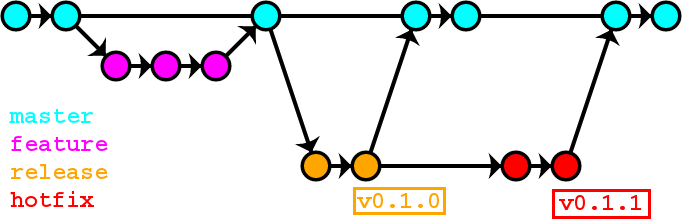
\includegraphics[width=0.8\textwidth]{img/git_branches.png}
        \end{center}
    \end{frame}

    \begin{frame}[t,fragile]{Git}
        \begin{itemize}
            \item{Track changes to your code}
            \item{Comment your changes}
            \item{Easily revert back to older versions}
            \item{Avoid/manage conflicts when working in teams}
            \item{Manage release versions and development versions}
            \item{Work on different branches at the same time}
        \end{itemize}
    \end{frame}

    \begin{frame}[t,fragile]{Git example}
        \begin{columns}[T]
            \column{0.5\textwidth}
            \begin{itemize}
                \item{Initialize a git repository}
                \item{Add files you want to include in a commit}
                \item{Create a commit for your selected changes}
                \item{Push changes to server}
            \end{itemize}
            \column{0.5\textwidth}
        \begin{bashenv}[\small]
git init
        \end{bashenv}
        \begin{bashenv}[\small]
git add changed_file.txt
        \end{bashenv}
        \begin{bashenv}[\small]
git commit
        \end{bashenv}
        \begin{bashenv}[\small]
git push
        \end{bashenv}
        \end{columns}
    \end{frame}

    \begin{frame}[t,fragile]{Sharing a repository}
        \begin{itemize}
            \item{You can use services like \emph{Github} or \emph{Gitlab} to collaborate
                with others on your project}
            \item{Or host your repositories yourself!}
                \begin{itemize}
                    \item{You can pull from/push to any server you can access via SSH}
                \end{itemize}
        \end{itemize}
    \end{frame}

    \section{Backup}
    \begin{frame}[t, fragile]{Borg Backup}
	    \begin{columns}[T]
		    \column{0.5\textwidth}
		    \begin{itemize}
			    \item Backup data
			    \item Does compression and deduplication automatically
			    \item Possibility to encrypt
			    \item Runs over ssh, network storage etc.
		    \end{itemize}
		    \column{0.5\textwidth}
		    \begin{center}
			    
\includegraphics[width=0.6\columnwidth]{img/borg_logo.png}
			    \vspace{2cm}
		    \end{center}
	    \end{columns}
    \end{frame}

    \begin{frame}[t, fragile]{Borg Example}
		    \vspace{0.5cm}
		    \begin{itemize}
			    \item Repos are collections of backups
			    \item Create new backups with \texttt{borg create}
			    \item Restore files with \texttt{borg extract <archive>}
		    \end{itemize}
		    \vspace{0.5cm}
		    \begin{bashenv}[\scriptsize]
[luke@host ~]$ borg init --encryption=repokey /path/to/repo
Enter passphrase:
Repeat passphrase:
[luke@host ~]$ borg create /path/to/repo
[luke@host ~]$ borg create --stats /path/to/repo::Backup1 ~/dir_to_backup
[luke@host ~]$ borg create --stats /path/to/repo::Backup2 ~/dir_to_backup
[luke@host ~]$ borg extract /path/to/repo::Backup1
		    \end{bashenv}
		    \vspace{0.5cm}
    \end{frame}

    \section{Epilogue}

    \begin{frame}[t,fragile]{Sources}
        \begin{itemize}
            \item Img 1
            \item Img 2
        \end{itemize}
    \end{frame}

    % \begin{frame}[t,fragile]{INSERT TITLE}
    %     \begin{columns}[T]
    %         \column{0.5\textwidth}
    %         \column{0.5\textwidth}
    %     \end{columns}
    % \end{frame}

\end{document}
